\chapter{Experiments}\label{chp:experiments}

In this chapter we'll benchmark a WebRTC-based video conferencing solution for our test cases, to get a sense of how a peer-to-peer architecture performs.


\section{Test Setup}

To benchmark appear.in, our WebRTC-based video conferencing solution of choice, we have utilized a small cluster of desktop computers with web cameras, running a recent version of Mozilla Firefox. The goal of the benchmark is to get a sense of how the application performs with regard to latency and bandwidth usage in our different test scenarios, and from that data observe how resources are shared among the nodes in a conversation.

WebRTC doesn't expose any \glspl{api} for accessing latency of a given stream, thus we had to improvise how to measure this. We settled for a solution based on having each node broadcast a timestamp in its video stream, which each receiving node could then compare to their local time. As long as all the clocks are syncronized against the same NTP servers, they should be more than accurate enough to measure the different latencies observed in the system.

Practically this was accomplished by having each computer film a timer running on a separate computer, and run the same timer locally. A screenshot was taken regularly through the test run, enabling extraction of the time as sent by each of the other nodes later. See \autoref{fig:example-screenshot} for an example of how the screenshots looked.

\begin{figure}
    \centering
    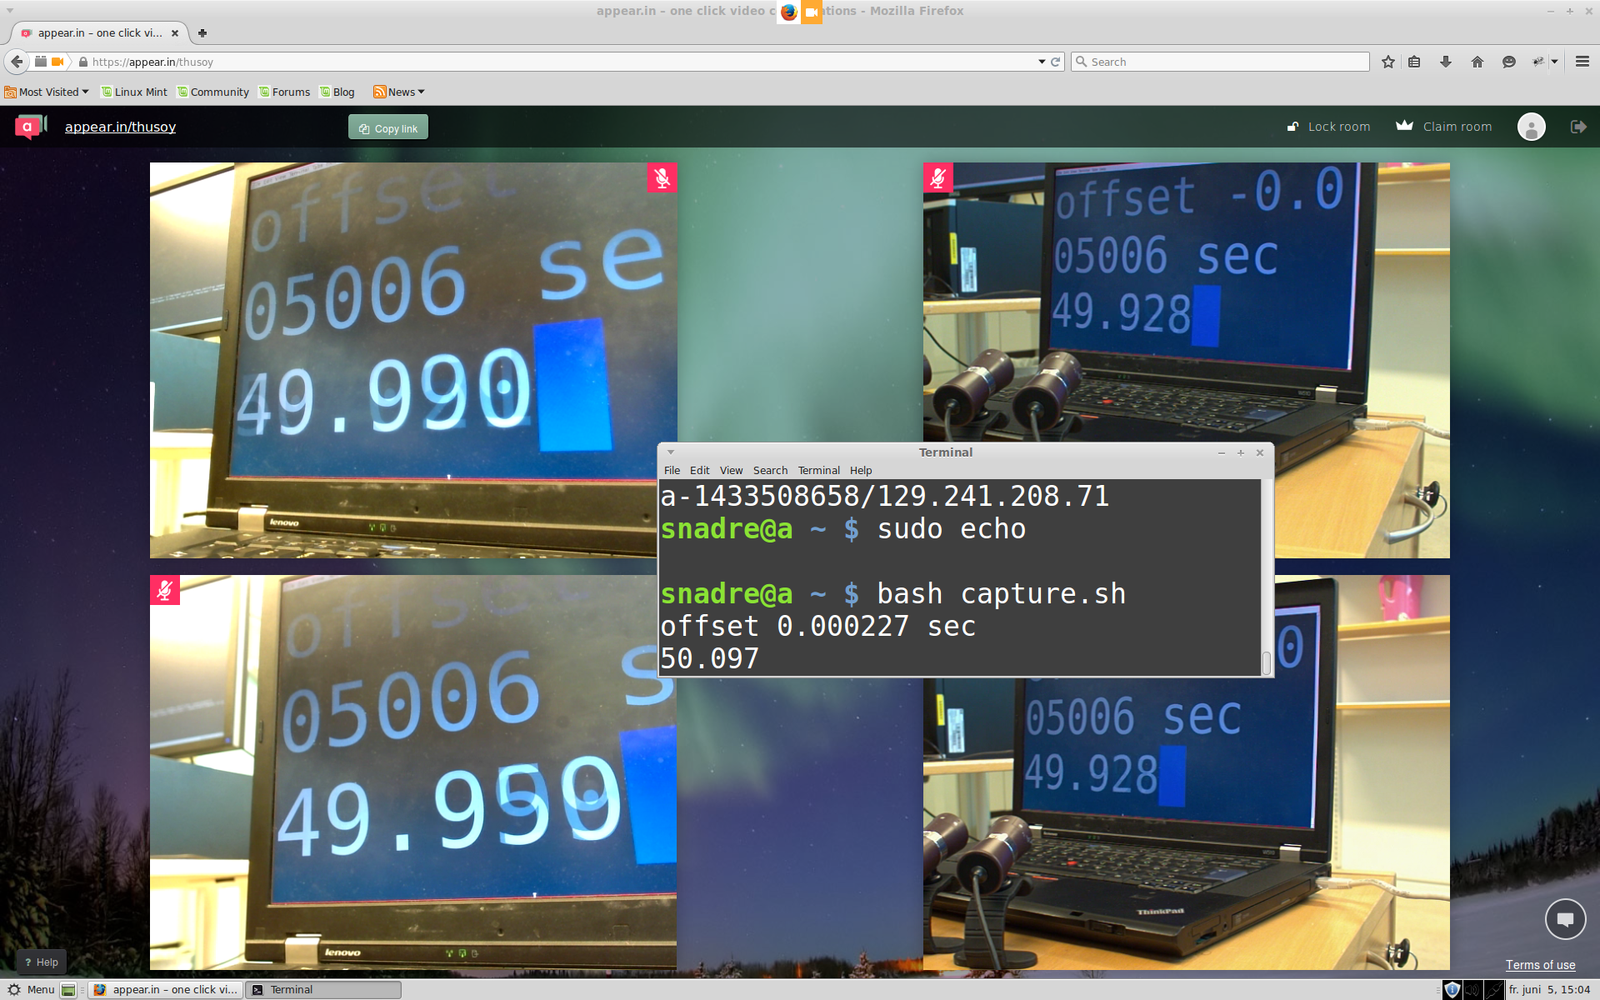
\includegraphics[width=.7\textwidth]{example-screenshot}
    \caption{An example screenshot from a test run on node A. The nodes are, from top left and clockwise, A, C, B and D. We can see from the difference between the local timestamp and A's own video stream that there's about 75ms of processing time in the browser before the image is sent (if we round A up to the almost visible 50.021 timestamp), and that the latencies from the other nodes are 31ms, 93ms and 93ms for B, C, and D, respectively.}
    \label{fig:example-screenshot}
\end{figure}

Bandwidth usage was measured by running \texttt{tcpdump} throughout the test run, and later extracting sent and received data with \texttt{tshark}.

To configure the cluster according to the different test cases, we utilized the Linux traffic control utility \texttt{tc}, which is capable of rate-limiting incoming and outgoing traffic, as well as delaying traffic destined for certain hosts. A small script was developed to act as a glue layer between a representation of a network and \texttt{tc}, making configuration repeatable and easily parametrized. The script is included in \autoref{chp:apply-case}.

Thus, applying a given test case is completely independent of the actual network utilized in the test cluster, keeping all intelligence on the nodes themselves. This removed the need for expensive routers or having to customize the application code, thus making the method application agnostic and applicable to any peer-to-peer solution, not just appear.in.

In contrast to most other video conferencing solutions, appear.in displays a node's own video stream just as big as the other streams in the conversation. This enables us to get a sense of how much time the browser spends processing the incoming video stream, as we can estimate this as the difference between the local timestamp and the timestamp of your own video stream as displayed in the browser. Since we're not benchmarking CPU usage in these tests, we can subtract this difference from the observed latencies between the other nodes, to only look at latencies originating in the network stack.

Ideally, testing would be automated and not require a running graphical environment, to allow it to be tested using remote servers. This could be possible using \texttt{node-webrtc}\footnote{\url{https://github.com/js-platform/node-webrtc}} or running a browser in a fake framebuffer like \texttt{Xvfb}\footnote{\url{http://www.x.org/releases/X11R7.6/doc/man/man1/Xvfb.1.xhtml}} and faking out a media stream\footnote{Chrome: \texttt{-{}-use-fake-device-for-media-stream}, Firefox: \texttt{getUserMedia(\{fake: true, <...>\})}. More info at \url{http://images.tmcnet.com/expo/webrtc-conference/presentations/san-jose-14/D3-2_Testing_v2_2.pdf}}. It is thus probably possible to automate this, but was considered out of scope for this thesis.


\section{Caveats}

Our method is accurate in the sense that latencies observed are the actual end-to-end latencies that users would observe, but the precision of the timing values observed is not on the millisecond level we'd prefer. This is due to a number of factors, most notably the refresh rate of the screen running the timer and the framerate of the video, limiting the precision to $1s/60\approx17ms$ and $1s/30\approx33ms$ respectively. However, we can surpass this precision by averaging several samples taken during the test run, which is why we take several screenshots for each test case, once every 10s for at least a minute. The standard deviation of the measurements is reported in the graphs included later in this chapter, which should give some indication towards how accurate the average is.

Taking several samples to improve accuracy leads us to another weakness, which is the manual interpretation of the screenshots. Due to the frequency-related issues discussed above, many of the images include timestamps that are blurred, as the camera captured two underlying screen updates in the same frame, as shown in \autoref{fig:blurred-capture}.

\begin{figure}
    \centering
    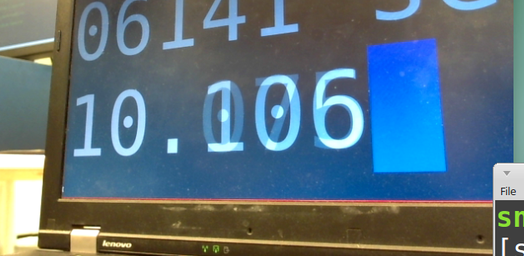
\includegraphics[width=.7\textwidth]{blurred-capture}
    \caption{A screenshot where a node has sent two overlaying timestamps. In this case interpreted as 10.106, which is reasonable as it's close to a 33ms increase from the previous 10.075.}
    \label{fig:blurred-capture}
\end{figure}

In general for these cases, the recorded timestamp was consistently interpreted to be the latest of what could be distinguished in the screenshot.

Even assuming that the timestamps are comprehensible and fairly accurate, there's still a possibility of human error when lots of numbers has to be recorded in this way. To minimize the risk of any mistyped numbers making it into the dataset, any number outside 1.5 standard deviations of the mean (a range which should include \todo{find actual range covered}80\% of the numbers observed) was verified once more. There's still a chance of smaller errors making it into the dataset, but we assume that these are small enough and distributed evenly among the nodes to not significantly influence any conclusions drawn.

For measuring bandwidth utilization between nodes, our method of using \texttt{tcpdump} is not entirely satisfactory, as there's no way to report actual \emph{consumed} bandwidth by the application. This is due to the traffic control features of the Linux kernel lying above where \texttt{libpcap}, the library that performs packet capture for \texttt{tcpdump}, listens in the network stack, meaning any incoming bandwidth reported will be before the rate limiting performed by \texttt{tc}. Thus, \texttt{tcpdump} cannot report the bandwidth actually consumed by application, only what was actually received by the network interface. Nonetheless, the bandwidth \emph{sent} by each node is what was actually sent by the application, but there's no guarantee that the node was actually capable of consuming it all. This is good enough for us though, as we can aggregate the data sent by all nodes to determine how saturated a given node's network link is.

While the method itself is application-agnostic, configuring nodes the way we do is not suitable for testing other architectures, such as the ones used by Hangouts and Skype. This is unfortunate, as a performance comparison between the different architectures would have been very interesting, but without running a local instance of the architecture under test, there's no way to achieve the internode latencies we desire. This follows from observing that if node A sends her video stream to a Google server, there's no way for her to signal to Google that when the stream is broadcast to nodes B and C, B's stream should be delayed by $x$ms, and the stream to C should be delayed $y$ms. It's also not possible for B and C to apply this latency on the receiving side, as they'd have to split the incoming stream for Google into separate streams for each of the transmitting nodes, which would require both getting access to the DTLS keys used by the web browser to encrypt the traffic, and being capable of splitting the stream and rejoining it again without interfering with the browser.


\section{Method}\label{sec:method}

(screensharing scrapped due to framerate artifically limited too severly, did not run any custom code since the solution needed to be (relatively) service agnostic, and could not modify code since it would need to be tagged in the video stream somehow. Some for appear.in, would need to be included in the sdp stream, and extracted -> way too much work).


\section{Results}

To get a sense of how appear.in performs under optimal conditions, a test run was performed with 3, 4 and 7 nodes in a conversation, without any traffic shaping. We would expect both bandwidth and latencies to be fairly even among all the nodes, as the only thing different between them is the time they entered the conversation. Since they were given some time to stabilize before the measurements was started, some fairness should have been achieved.

As we see in \autoref{fig:vanilla-3p}, bitrates between the nodes are identical, as expected. From the latency measurements there seems to be a slight inclination towards the latest arriving node having somewhat higher latencies outgoing, but the difference is negligible in practice.

\begin{figure}
    \centering
    \begin{subfigure}[t]{.48\textwidth}
        \centering
        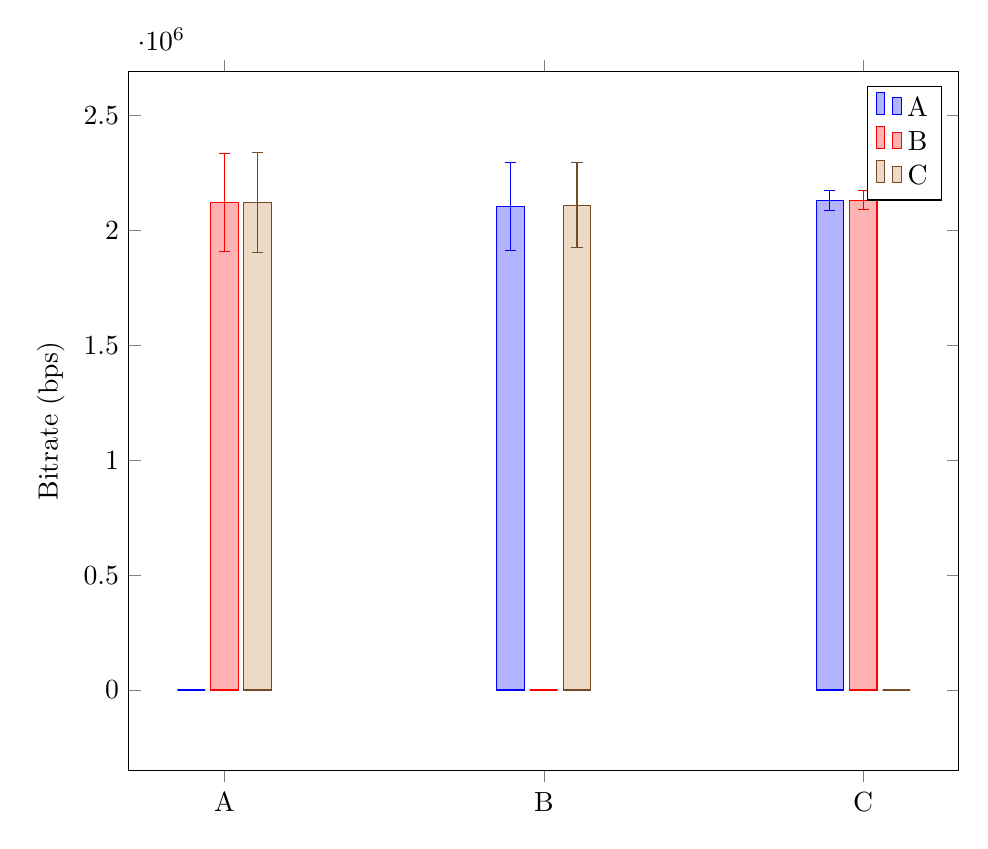
\begin{tikzpicture}
        \begin{axis}[
            ybar,
            ylabel=Bitrate (bps),
            xtick=data,
            width=\textwidth,
            symbolic x coords={A,B,C},
            enlargelimits=0.15
            ]

            %% Traffic received by A
            \addplot+[error bars/.cd,y dir=both, y explicit]
            coordinates{
                (A,0) +- (0.0, 0)
                (B,2103841) +- (0.0, 190915)
                (C,2130058) +- (0.0, 44133)};

            %% Traffic received by B
            \addplot+[error bars/.cd,y dir=both, y explicit]
            coordinates{
                (A,2121908) +- (0.0, 212606)
                (B,0) +- (0.0, 0)
                (C,2130480) +- (0.0, 41317)};

            %% Traffic received by C
            \addplot+[error bars/.cd,y dir=both, y explicit]
            coordinates{
                (A,2121362) +- (0.0, 217821)
                (B,2108437) +- (0.0, 184826)
                (C,0) +- (0.0, 0)};

            \legend{A, B, C}
        \end{axis}
        \end{tikzpicture}
        \subcaption{Outgoing traffic from each node}
    \end{subfigure}
    \hfill
    \begin{subfigure}[t]{.48\textwidth}
        \centering
        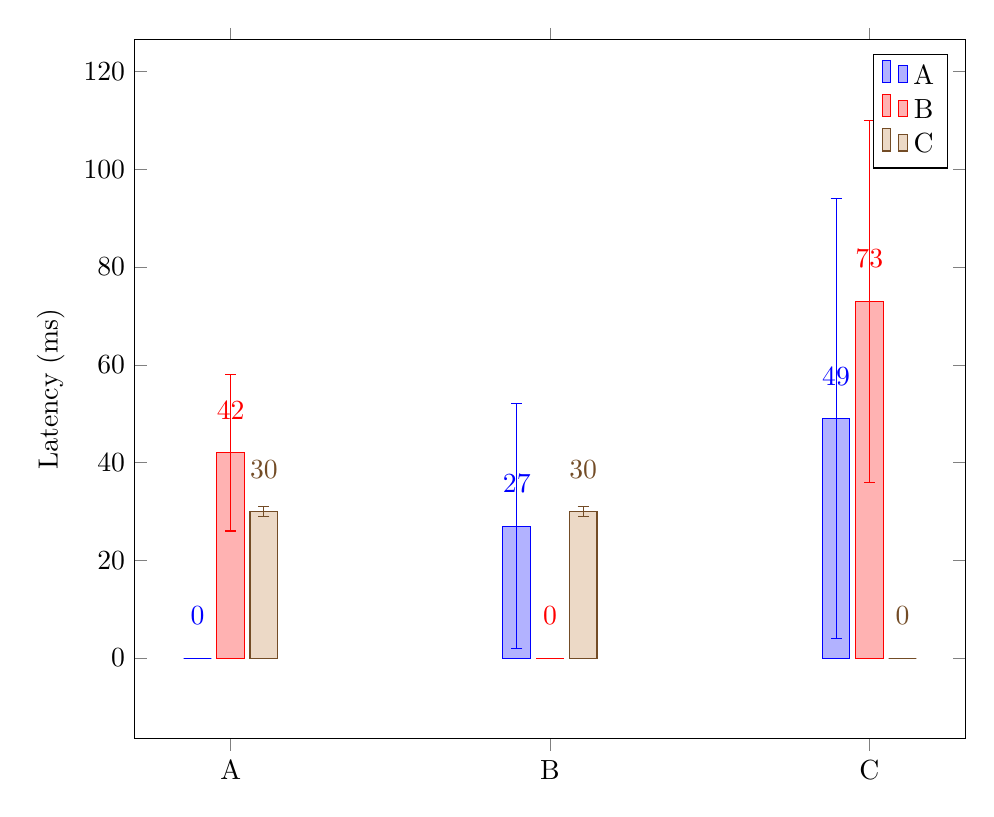
\begin{tikzpicture}
        \begin{axis}[
            ybar,
            compat=newest,
            ylabel=Latency (ms),
            xtick=data,
            width=\textwidth,
            symbolic x coords={A,B,C},
            enlargelimits=0.15,
            nodes near coords=\raisebox{.3cm}{\pgfmathprintnumber{\pgfplotspointmeta}}
            ]

            \addplot+[error bars/.cd,y dir=both, y explicit]
            coordinates{
                (A,0) +- (0.0, 0)
                (B,27) +- (0.0, 25)
                (C,49) +- (0.0, 45)};

            \addplot+[error bars/.cd,y dir=both, y explicit]
            coordinates{
                (A,42) +- (0.0, 16)
                (B,0) +- (0.0, 0)
                (C,73) +- (0.0, 37)};

            \addplot+[error bars/.cd,y dir=both, y explicit]
            coordinates{
                (A,30) +- (0.0, 1)
                (B,30) +- (0.0, 1)
                (C,0) +- (0.0, 0)};

            \legend{A, B, C}
        \end{axis}
        \end{tikzpicture}
        \subcaption{Outgoing latencies for each node}
    \end{subfigure}
    \caption{Test results for three nodes without traffic shaping}
    \label{fig:vanilla-3p}
\end{figure}

Adding another node to the mix, we get the results as shown in \autoref{fig:vanilla-4p}. We see that the bandwidth between the nodes is the same 2.1Mpbs that we saw when there was only three nodes in the conversation, which we can assume is the default transmit bitrate for appear.in. We can also see the same phenomena as in the three node case, that the later arrivals tend to have a slightly higher latency to the nodes first to arrive in the conversation. However, the later nodes (C and D) does not display this phenomena between themselves, thus since all the observations are within one standard deviation of each other we'll not spend any more time investigating this.


\begin{figure}
    \centering
    \begin{subfigure}[t]{.9\textwidth}
        \centering
        \begin{tikzpicture}
        \begin{axis}[
            ybar,
            ylabel=Bitrate (bps),
            xtick=data,
            width=\textwidth,
            bar width=10,
            height=240,
            symbolic x coords={A,B,C,D},
            enlargelimits=0.15
            ]

            %% Traffic received by A
            \addplot+[error bars/.cd,y dir=both, y explicit]
            coordinates{
                (A,0) +- (0.0, 0)
                (B,2108732) +- (0.0, 122299)
                (C,2122345) +- (0.0, 102937)
                (D,2129951) +- (0.0, 31694)};

            %% Traffic received by B
            \addplot+[error bars/.cd,y dir=both, y explicit]
            coordinates{
                (A,2114546) +- (0.0, 77200)
                (B,0) +- (0.0, 0)
                (C,2121893) +- (0.0, 110336)
                (D,2130755) +- (0.0, 31111)};

            %% Traffic received by C
            \addplot+[error bars/.cd,y dir=both, y explicit]
            coordinates{
                (A,2114445) +- (0.0, 61198)
                (B,2109369) +- (0.0, 133375)
                (C,0) +- (0.0, 0)
                (D,2130008) +- (0.0, 32655)};

            %% Traffic received by D
            \addplot+[error bars/.cd,y dir=both, y explicit]
            coordinates{
                (A,2115163) +- (0.0, 72349)
                (B,2108265) +- (0.0, 124281)
                (C,2122517) +- (0.0, 106959)
                (D,0) +- (0.0, 0)};

            \legend{A, B, C, D}
        \end{axis}
        \end{tikzpicture}
        \subcaption{Outgoing traffic from each node}
    \end{subfigure}
    \begin{subfigure}[t]{.9\textwidth}
        \centering
        \begin{tikzpicture}
        \begin{axis}[
            ybar,
            compat=newest,
            ylabel=Latency (ms),
            xtick=data,
            width=\textwidth,
            symbolic x coords={A,B,C,D},
            bar width=10,
            height=240,
            enlargelimits=0.15,
            nodes near coords=\raisebox{.3cm}{\pgfmathprintnumber{\pgfplotspointmeta}}
            ]

            \addplot+[error bars/.cd,y dir=both, y explicit]
            coordinates{
                (A,0) +- (0.0, 0)
                (B,40) +- (0.0, 30)
                (C,60) +- (0.0, 37)
                (D,68) +- (0.0, 25)};

            \addplot+[error bars/.cd,y dir=both, y explicit]
            coordinates{
                (A,51) +- (0.0, 23)
                (B,0) +- (0.0, 0)
                (C,65) +- (0.0, 27)
                (D,65) +- (0.0, 27)};

            \addplot+[error bars/.cd,y dir=both, y explicit]
            coordinates{
                (A,15) +- (0.0, 21)
                (B,15) +- (0.0, 21)
                (C,0) +- (0.0, 0)
                (D,30) +- (0.0, 0)};

            \addplot+[error bars/.cd,y dir=both, y explicit]
            coordinates{
                (A,30) +- (0.0, 27)
                (B,15) +- (0.0, 16)
                (C,37) +- (0.0, 12)
                (D,0) +- (0.0, 0)};

            \legend{A, B, C, D}
        \end{axis}
        \end{tikzpicture}
        \subcaption{Outgoing latencies for each node}
    \end{subfigure}
    \caption{Test results for four nodes without traffic shaping}
    \label{fig:vanilla-4p}
\end{figure}

In the final test without traffic shaping, we step it up to seven nodes in the conversation. The results can be seen in \autoref{fig:vanilla-7p}, and largely mirror what we saw in the smaller experiements. Latencies are a bit higher, which can probably be expected due to the increase in traffic, and apart from a bandwidth deviation on node E, all nodes continue transmitting on the previously observed 2.1Mbps. Why node E's behavior is worse than the other nodes are unknown, but it could be related to node E being on a busier subnet than the other nodes (E was the only node in the test cluster on its subnet).


\begin{figure}
    \centering
    \begin{subfigure}[t]{\textwidth}
        \centering
        \begin{tikzpicture}
        \begin{axis}[
            ybar,
            ylabel=Bitrate (bps),
            xtick=data,
            width=\textwidth,
            bar width=3,
            height=240,
            symbolic x coords={A,B,C,D,E,F,G},
            enlargelimits=0.10
            ]

            %% Traffic received by A
            \addplot+[error bars/.cd,y dir=both, y explicit]
            coordinates{
                (A,0) +- (0.0, 0)
                (B,2130034) +- (0.0, 51733)
                (C,2128127) +- (0.0, 58288)
                (D,2119439) +- (0.0, 153797)
                (E,1516049) +- (0.0, 530232)
                (F,2120354) +- (0.0, 141506)
                (G,2123271) +- (0.0, 92795)};

            %% Traffic received by B
            \addplot+[error bars/.cd,y dir=both, y explicit]
            coordinates{
                (A,2120036) +- (0.0, 154055)
                (B,0) +- (0.0, 0)
                (C,2127250) +- (0.0, 56219)
                (D,2119188) +- (0.0, 160008)
                (E,1453429) +- (0.0, 532842)
                (F,2120152) +- (0.0, 135732)
                (G,2122753) +- (0.0, 90278)};

            %% Traffic received by C
            \addplot+[error bars/.cd,y dir=both, y explicit]
            coordinates{
                (A,2120665) +- (0.0, 150280)
                (B,2130031) +- (0.0, 45591)
                (C,0) +- (0.0, 0)
                (D,2119627) +- (0.0, 152410)
                (E,1543173) +- (0.0, 562049)
                (F,2119490) +- (0.0, 148053)
                (G,2123174) +- (0.0, 96945)};

            %% Traffic received by D
            \addplot+[error bars/.cd,y dir=both, y explicit]
            coordinates{
                (A,2121283) +- (0.0, 153257)
                (B,2128463) +- (0.0, 53731)
                (C,2127889) +- (0.0, 55279)
                (D,0) +- (0.0, 0)
                (E,1676161) +- (0.0, 480970)
                (F,2119602) +- (0.0, 138893)
                (G,2122794) +- (0.0, 89433)};

            %% Traffic received by E
            \addplot+[error bars/.cd,y dir=both, y explicit]
            coordinates{
                (A,2121256) +- (0.0, 153063)
                (B,2130945) +- (0.0, 51320)
                (C,2127847) +- (0.0, 65898)
                (D,2119733) +- (0.0, 158459)
                (E,0) +- (0.0, 0)
                (F,2119668) +- (0.0, 134677)
                (G,2123002) +- (0.0, 95431)};

            %% Traffic received by F
            \addplot+[error bars/.cd,y dir=both, y explicit]
            coordinates{
                (A,2121177) +- (0.0, 151443)
                (B,2132365) +- (0.0, 44058)
                (C,2127846) +- (0.0, 63152)
                (D,2119672) +- (0.0, 153872)
                (E,1094226) +- (0.0, 385404)
                (F,0) +- (0.0, 0)
                (G,2123497) +- (0.0, 96151)};

            %% Traffic received by G
            \addplot+[error bars/.cd,y dir=both, y explicit]
            coordinates{
                (A,2120585) +- (0.0, 155610)
                (B,2132137) +- (0.0, 46317)
                (C,2130083) +- (0.0, 64279)
                (D,2119292) +- (0.0, 154126)
                (E,1602265) +- (0.0, 482579)
                (F,2120748) +- (0.0, 141272)
                (G,0) +- (0.0, 0)};

            \legend{A, B, C, D, E, F, G}
        \end{axis}
        \end{tikzpicture}
        \subcaption{Outgoing traffic from each node}
    \end{subfigure}
    \begin{subfigure}[t]{\textwidth}
        \centering
        \begin{tikzpicture}
        \begin{axis}[
            ybar,
            compat=newest,
            ylabel=Latency (ms),
            xtick=data,
            width=\textwidth,
            symbolic x coords={A,B,C,D,E,F,G},
            bar width=3,
            height=240,
            enlargelimits=0.10,
            nodes near coords=\raisebox{.3cm}{\pgfmathprintnumber{\pgfplotspointmeta}}
            ]

            \addplot+[error bars/.cd,y dir=both, y explicit]
            coordinates{
                (A,0) +- (0.0, 0)
                (B,60) +- (0.0, 31)
                (C,90) +- (0.0, 36)
                (D,88) +- (0.0, 41)
                (E,169) +- (0.0, 29)
                (F,34) +- (0.0, 28)
                (G,47) +- (0.0, 17)};

            \addplot+[error bars/.cd,y dir=both, y explicit]
            coordinates{
                (A,52) +- (0.0, 23)
                (B,0) +- (0.0, 0)
                (C,97) +- (0.0, 52)
                (D,91) +- (0.0, 17)
                (E,144) +- (0.0, 42)
                (F,30) +- (0.0, 18)
                (G,52) +- (0.0, 23)};

            \addplot+[error bars/.cd,y dir=both, y explicit]
            coordinates{
                (A,20) +- (0.0, 17)
                (B,20) +- (0.0, 17)
                (C,0) +- (0.0, 0)
                (D,71) +- (0.0, 18)
                (E,112) +- (0.0, 18)
                (F,20) +- (0.0, 17)
                (G,40) +- (0.0, 17)};

            \addplot+[error bars/.cd,y dir=both, y explicit]
            coordinates{
                (A,22) +- (0.0, 15)
                (B,15) +- (0.0, 17)
                (C,94) +- (0.0, 48)
                (D,0) +- (0.0, 0)
                (E,123) +- (0.0, 24)
                (F,15) +- (0.0, 17)
                (G,15) +- (0.0, 17)};

            \addplot+[error bars/.cd,y dir=both, y explicit]
            coordinates{
                (A,76) +- (0.0, 27)
                (B,86) +- (0.0, 24)
                (C,122) +- (0.0, 34)
                (D,126) +- (0.0, 23)
                (E,0) +- (0.0, 0)
                (F,61) +- (0.0, 19)
                (G,65) +- (0.0, 12)};

            \addplot+[error bars/.cd,y dir=both, y explicit]
            coordinates{
                (A,46) +- (0.0, 17)
                (B,51) +- (0.0, 25)
                (C,102) +- (0.0, 25)
                (D,97) +- (0.0, 23)
                (E,198) +- (0.0, 80)
                (F,0) +- (0.0, 0)
                (G,56) +- (0.0, 12)};

            \addplot+[error bars/.cd,y dir=both, y explicit]
            coordinates{
                (A,47) +- (0.0, 35)
                (B,64) +- (0.0, 24)
                (C,102) +- (0.0, 14)
                (D,95) +- (0.0, 35)
                (E,146) +- (0.0, 33)
                (F,47) +- (0.0, 31)
                (G,0) +- (0.0, 0)};

            \legend{A, B, C, D, E, F, G}
        \end{axis}
        \end{tikzpicture}
        \subcaption{Outgoing latencies for each node}
    \end{subfigure}
    \caption{Test results for seven nodes without traffic shaping}
    \label{fig:vanilla-7p}
\end{figure}




\todo[inline]{[minor] If time, define custom color set for graphing, based possibly either on solarized or http://clrs.cc/}
\todo{Gather some metrics from running the implementation in a prod environment}

For our first test case, "Asia", the bandwidth utilized by each node is shown in \autoref{fig:asia-bitrate}.

\begin{figure}
    \centering
    \begin{subfigure}[t]{.48\textwidth}
        \centering
        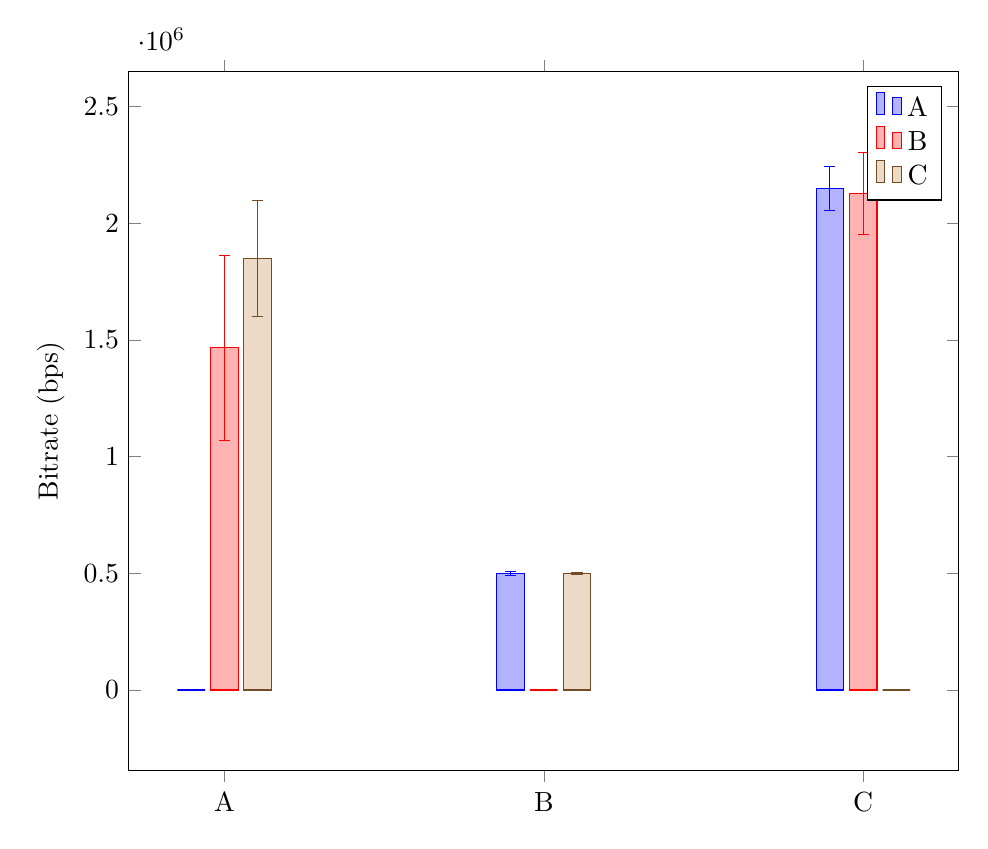
\begin{tikzpicture}
        \begin{axis}[
            ybar,
            ylabel=Bitrate (bps),
            xtick=data,
            width=\textwidth,
            symbolic x coords={A,B,C},
            enlargelimits=0.15
            ]
            %% Traffic received by A
            \addplot+[error bars/.cd,y dir=both, y explicit]
            coordinates{
                (A,0) +- (0.0, 0)
                (B,499012) +- (0.0, 7163)
                (C,2146920) +- (0.0, 94119)};

            %% Traffic received by B
            \addplot+[error bars/.cd,y dir=both, y explicit]
            coordinates{
                (A,1466045) +- (0.0, 396215)
                (B,0) +- (0.0, 0)
                (C,2128002) +- (0.0, 175433)};

            %% Traffic received by C
            \addplot+[error bars/.cd,y dir=both, y explicit]
            coordinates{
                (A,1847944) +- (0.0, 247449)
                (B,498988) +- (0.0, 5709)
                (C,0) +- (0.0, 0)};
            \legend{A, B, C}
        \end{axis}
        \end{tikzpicture}
        \subcaption{Outgoing traffic from each node}
    \end{subfigure}
    \hfill
    \begin{subfigure}[t]{.48\textwidth}
        \centering
        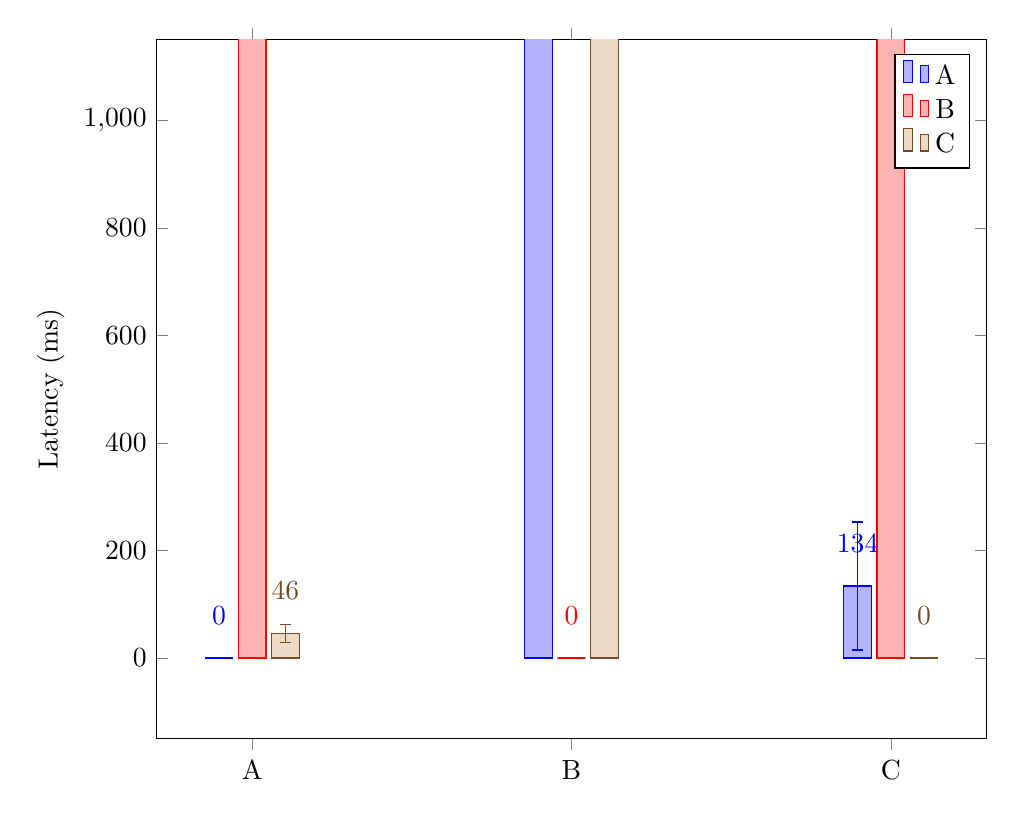
\begin{tikzpicture}
        \begin{axis}[
            ybar,
            compat=newest,
            ylabel=Latency (ms),
            xtick=data,
            ymax=1000,
            width=\textwidth,
            symbolic x coords={A,B,C},
            enlargelimits=0.15,
            nodes near coords=\raisebox{.3cm}{\pgfmathprintnumber{\pgfplotspointmeta}}
            ]

            \addplot+[error bars/.cd,y dir=both, y explicit]
            coordinates{
                (A,0) +- (0.0, 0)
                (B,25186) +- (0.0, 8743)
                (C,134) +- (0.0, 119)};

            \addplot+[error bars/.cd,y dir=both, y explicit]
            coordinates{
                (A,47731) +- (0.0, 23234)
                (B,0) +- (0.0, 0)
                (C,47752) +- (0.0, 23219)};

            \addplot+[error bars/.cd,y dir=both, y explicit]
            coordinates{
                (A,46) +- (0.0, 17)
                (B,24052) +- (0.0, 7647)
                (C,0) +- (0.0, 0)};

            \legend{A, B, C}
        \end{axis}
        \end{tikzpicture}
        \subcaption{Outgoing latencies for each node}
    \end{subfigure}
    \caption{Test results for the "asia" test case.}
    \label{fig:asia-bitrate}
\end{figure}

\begin{figure}
    \centering
    \begin{subfigure}[t]{.9\textwidth}
        \centering
        \begin{tikzpicture}
        \begin{axis}[
            ybar,
            ylabel=Bitrate (bps),
            xtick=data,
            width=\textwidth,
            bar width=10,
            height=240,
            symbolic x coords={A,B,C,D},
            enlargelimits=0.15
            ]
            %% Traffic received by A
            \addplot+[error bars/.cd,y dir=both, y explicit]
            coordinates{
                (A,0) +- (0.0, 0)
                (B,2132647) +- (0.0, 193663)
                (C,1753202) +- (0.0, 229020)
                (D,997887) +- (0.0, 106031)};

            %% Traffic received by B
            \addplot+[error bars/.cd,y dir=both, y explicit]
            coordinates{
                (A,2138074) +- (0.0, 95442)
                (B,0) +- (0.0, 0)
                (C,1938956) +- (0.0, 238021)
                (D,997355) +- (0.0, 103922)};

            %% Traffic received by C
            \addplot+[error bars/.cd,y dir=both, y explicit]
            coordinates{
                (A,2151129) +- (0.0, 116239)
                (B,2068979) +- (0.0, 190976)
                (C,0) +- (0.0, 0)
                (D,999131) +- (0.0, 102965)};

            %% Traffic received by D
            \addplot+[error bars/.cd,y dir=both, y explicit]
            coordinates{
                (A,2161007) +- (0.0, 128042)
                (B,2165180) +- (0.0, 158016)
                (C,2153238) +- (0.0, 218063)
                (D,0) +- (0.0, 0)};
            \legend{A, B, C, D}
        \end{axis}
        \end{tikzpicture}
        \subcaption{Outgoing traffic from each node}
    \end{subfigure}
    \begin{subfigure}[t]{.9\textwidth}
        \centering
        \begin{tikzpicture}
        \begin{axis}[
            ybar,
            ylabel=Latency (ms),
            xtick=data,
            width=\textwidth,
            ymax=1000,
            bar width=10,
            height=240,
            symbolic x coords={A,B,C,D},
            enlargelimits=0.15,
            nodes near coords=\raisebox{.3cm}{\pgfmathprintnumber{\pgfplotspointmeta}}
            ]

            \addplot+[error bars/.cd,y dir=both, y explicit]
            coordinates{
                (A,0) +- (0.0, 0)
                (B,61) +- (0.0, 19)
                (C,252) +- (0.0, 46)
                (D,16168) +- (0.0, 0)};

            \addplot+[error bars/.cd,y dir=both, y explicit]
            coordinates{
                (A,54) +- (0.0, 23)
                (B,0) +- (0.0, 0)
                (C,277) +- (0.0, 27)
                (D,11041) +- (0.0, 0)};

            \addplot+[error bars/.cd,y dir=both, y explicit]
            coordinates{
                (A,140) +- (0.0, 70)
                (B,179) +- (0.0, 71)
                (C,0) +- (0.0, 0)
                (D,15526) +- (0.0, 0)};

            \addplot+[error bars/.cd,y dir=both, y explicit]
            coordinates{
                (A,4683) +- (0.0, 0)
                (B,3437) +- (0.0, 0)
                (C,7750) +- (0.0, 0)
                (D,0) +- (0.0, 0)};

            \legend{A, B, C, D}
        \end{axis}
        \end{tikzpicture}
        \subcaption{Outgoing latencies for each node}
    \end{subfigure}
    \caption{Test results for the "standup" test case.}
\end{figure}


\begin{figure}
    \centering
    \begin{subfigure}[t]{\textwidth}
        \centering
        \begin{tikzpicture}
        \begin{axis}[
            ybar,
            ylabel=Bitrate (bps),
            xtick=data,
            width=\textwidth,
            bar width=3,
            height=240,
            symbolic x coords={A,B,C,D,E,F,G},
            enlargelimits=0.10
            ]

            %% Traffic received by A
            \addplot+[error bars/.cd,y dir=both, y explicit]
            coordinates{
                (A,0) +- (0.0, 0)
                (B,2122914) +- (0.0, 103365)
                (C,1335840) +- (0.0, 353924)
                (D,1433026) +- (0.0, 446130)
                (E,1326235) +- (0.0, 332558)
                (F,1878705) +- (0.0, 235041)
                (G,663701) +- (0.0, 149691)};

            %% Traffic received by B
            \addplot+[error bars/.cd,y dir=both, y explicit]
            coordinates{
                (A,2113784) +- (0.0, 199511)
                (B,0) +- (0.0, 0)
                (C,1313147) +- (0.0, 349341)
                (D,1494177) +- (0.0, 441797)
                (E,1391230) +- (0.0, 311771)
                (F,1971327) +- (0.0, 168470)
                (G,662717) +- (0.0, 190168)};

            %% Traffic received by C
            \addplot+[error bars/.cd,y dir=both, y explicit]
            coordinates{
                (A,2122002) +- (0.0, 198341)
                (B,2130824) +- (0.0, 105922)
                (C,0) +- (0.0, 0)
                (D,1548639) +- (0.0, 413383)
                (E,2031425) +- (0.0, 396762)
                (F,2140084) +- (0.0, 83964)
                (G,661920) +- (0.0, 150000)};

            %% Traffic received by D
            \addplot+[error bars/.cd,y dir=both, y explicit]
            coordinates{
                (A,2128216) +- (0.0, 198663)
                (B,2138372) +- (0.0, 107683)
                (C,1320751) +- (0.0, 360809)
                (D,0) +- (0.0, 0)
                (E,1817435) +- (0.0, 480759)
                (F,2132568) +- (0.0, 82901)
                (G,663245) +- (0.0, 188153)};

            %% Traffic received by E
            \addplot+[error bars/.cd,y dir=both, y explicit]
            coordinates{
                (A,2126240) +- (0.0, 216448)
                (B,2122724) +- (0.0, 139635)
                (C,1283979) +- (0.0, 344558)
                (D,1490125) +- (0.0, 398365)
                (E,0) +- (0.0, 0)
                (F,2125011) +- (0.0, 82898)
                (G,663739) +- (0.0, 148425)};

            %% Traffic received by F
            \addplot+[error bars/.cd,y dir=both, y explicit]
            coordinates{
                (A,1906059) +- (0.0, 236152)
                (B,1902141) +- (0.0, 245489)
                (C,1331865) +- (0.0, 353555)
                (D,1501551) +- (0.0, 438808)
                (E,1925676) +- (0.0, 439134)
                (F,0) +- (0.0, 0)
                (G,663802) +- (0.0, 188379)};

            %% Traffic received by G
            \addplot+[error bars/.cd,y dir=both, y explicit]
            coordinates{
                (A,2125677) +- (0.0, 216945)
                (B,2136130) +- (0.0, 129170)
                (C,1366067) +- (0.0, 330189)
                (D,1513765) +- (0.0, 372789)
                (E,1757906) +- (0.0, 510980)
                (F,2131239) +- (0.0, 93299)
                (G,0) +- (0.0, 0)};

            \legend{A, B, C, D, E, F, G}
        \end{axis}
        \end{tikzpicture}
        \subcaption{Outgoing traffic from each node}
    \end{subfigure}
    \begin{subfigure}[t]{\textwidth}
        \centering
        \begin{tikzpicture}
        \begin{axis}[
            ybar,
            compat=newest,
            ylabel=Latency (ms),
            ymax=1000,
            xtick=data,
            width=\textwidth,
            symbolic x coords={A,B,C,D,E,F,G},
            bar width=3,
            height=240,
            enlargelimits=0.10,
            nodes near coords=\raisebox{.3cm}{\pgfmathprintnumber{\pgfplotspointmeta}}
            ]

            \addplot+[error bars/.cd,y dir=both, y explicit]
            coordinates{
                (A,0) +- (0.0, 0)
                (B,71) +- (0.0, 16)
                (C,9720) +- (0.0, 0)
                (D,5845) +- (0.0, 0)
                (E,341) +- (0.0, 76)
                (F,1329) +- (0.0, 0)
                (G,12792) +- (0.0, 0)};

            \addplot+[error bars/.cd,y dir=both, y explicit]
            coordinates{
                (A,60) +- (0.0, 18)
                (B,0) +- (0.0, 0)
                (C,8163) +- (0.0, 0)
                (D,11178) +- (0.0, 0)
                (E,753) +- (0.0, 1038)
                (F,413) +- (0.0, 404)
                (G,19280) +- (0.0, 0)};

            \addplot+[error bars/.cd,y dir=both, y explicit]
            coordinates{
                (A,12) +- (0.0, 16)
                (B,6) +- (0.0, 13)
                (C,0) +- (0.0, 0)
                (D,9330) +- (0.0, 0)
                (E,2087) +- (0.0, 0)
                (F,2900) +- (0.0, 0)
                (G,27351) +- (0.0, 0)};

            \addplot+[error bars/.cd,y dir=both, y explicit]
            coordinates{
                (A,2074) +- (0.0, 0)
                (B,3056) +- (0.0, 0)
                (C,7300) +- (0.0, 0)
                (D,0) +- (0.0, 0)
                (E,250) +- (0.0, 138)
                (F,36) +- (0.0, 49)
                (G,20225) +- (0.0, 0)};

            \addplot+[error bars/.cd,y dir=both, y explicit]
            coordinates{
                (A,281) +- (0.0, 84)
                (B,1314) +- (0.0, 0)
                (C,9177) +- (0.0, 0)
                (D,10619) +- (0.0, 0)
                (E,0) +- (0.0, 0)
                (F,50038) +- (0.0, 0)
                (G,17236) +- (0.0, 0)};

            \addplot+[error bars/.cd,y dir=both, y explicit]
            coordinates{
                (A,2144) +- (0.0, 0)
                (B,1646) +- (0.0, 0)
                (C,11106) +- (0.0, 0)
                (D,4518) +- (0.0, 0)
                (E,140) +- (0.0, 33)
                (F,0) +- (0.0, 0)
                (G,18154) +- (0.0, 0)};

            \addplot+[error bars/.cd,y dir=both, y explicit]
            coordinates{
                (A,6158) +- (0.0, 0)
                (B,2336) +- (0.0, 0)
                (C,17100) +- (0.0, 0)
                (D,26423) +- (0.0, 0)
                (E,3564) +- (0.0, 0)
                (F,2965) +- (0.0, 0)
                (G,0) +- (0.0, 0)};

            \legend{A, B, C, D, E, F, G}
        \end{axis}
        \end{tikzpicture}
        \subcaption{Outgoing latencies for each node}
    \end{subfigure}
    \caption{Test results for the "friends" test case}
    \label{fig:friends}
\end{figure}
